\chapter{Methodology}

\section{Salinity Measurement Method}
A \gls{ctd} sensor, which measures salinity using conductivity, temperature and depth, was chosen as the salinity measurement device.
When choosing a measurement technique multiple factors needed to be considered.
Firstly, the salinity measurements are to be conducted in the Antarctic, where the environment, and remote nature of the area, make majority of the measurement methods unusable.
Secondly, the device would need to fit through an ice core hole with a diameter of $100mm$, and lastly, the device would need to be able to take continuous measurements.

\gls{ctd} sensors do not require sample collection, unlike chlorinity titration, gravimetric analysis and refractometry.
This removes both the need for sample collection and the challenges of sample degradation, storage and transport logistics.

Modern \gls{ctd} sensors are compact, and can easily be designed for specific space constraints.
This coupled with its deployments flexibility make it the preferred choice over methods, such as laboratory methods, which suffer from deployment constraints.
\gls{ctd} sensors allow for continuous realtime monitoring, a characteristic none of the the alternative methods provide.
The alternative methods either require sample collection, or cannot measure continuously.

\gls{ctd} instruments inherently measure conductivity, temperature and pressure simultaneously, providing salinity measurements with temperature and depth compensation, whereas laboratory methods measure salinity only, and require seperate temperature measurements.


These factors coupled with the researcher's significant experience with PCB design and electronics influenced the choice for a \gls{ctd} sensor.

\section{Electrode Design}
When measuring conductivity, choosing an electrode material plays a significant role in the accuracy of the measurements.
To get an accurate measurement of the resistance of the water, ideally, a electrode resistance of zero is required.
This would allow the resistance measurement to be entirely due to the resistance of the water.
Most conductive materials have conductivities of order $10^6 - 10^8 S/m$, which is negligible compared to sea (salt) water, which has an average conductivity of $3.31 S/m$~\cite{conductivities}\cite{ocean_conductivity_tyler}.
Preferably, the material with the highest conductivity, silver, would be used. However, conductivity is not the only factor considred when designing an electrode. 
The electrodes will be submerged in saltwater, which is highly corrosive. The material chosen will require high corrosive resistance. 
Silver, though having the highest conductivity, has a low corrosion resistance, and therefore cannot be used in this application~\cite{zhang_silver}.

Titanium is the material of choice for ocean-use~\cite{materials_ocean_structures}. It is essentially corrosion-free, and offers a conductivity of $2.68\times 10^{6}$~\cite{conductivities}.
However, titanium is expensive and fell out of the budget of this project.
Gold boasts both a high conductivity of $4.10\times 10^{7}$, higher than titanium but lower than silver, and a high corrosion resistance, making it an ideal choice.
Gold is also a commonly used material in electronic design, with it being used in \gls{pcb} manufacturing, to protect copper pads from corrosion.
This is done through a \gls{enig} plating process, where a layer of nickel is chemically deposited onto the exposed copper traces, to prevent the copper from oxidizing, and then a layer of gold is applied over the nickel through an emmersion process, to protect the nickel.
This process is significantly more expensive compared to standard \gls{pcb} manufacturing, however, it allowed for the use of gold electrodes, and therefore was factored into the budget. 

In order to utilise the \gls{enig} process a \gls{pcb} was used to design the gold electrodes.
This allowed the electrodes to be designed with a known area and seperation distance, allowing for accurate conductivity calculations.
A solder pad was used to design the portion of the \gls{pcb} that would act as the electrode, since it allowed the copper/gold to be exposed.
Then during manufacturing \gls{enig} was chosen as the surface finish, to achieve the gold finish.

The \gls{pcb} was designed to allow for easy calculation of the conductivity $\sigma$, using the equation below:
\begin{equation}\label{eqn:conductivity}
    \sigma = \frac{L}{RA}
\end{equation}

where $L$ is the distance between the electrodes, $R$ is the resistance of the water, and A is the cross-sectional area of the electrodes.
A square face of $20mm\times 20mm$ was chosen to allow for easy cross-sectional area calculations, and a distance of $10mm$ was chosen as the seperation distance.
This distance was chosen as it is close enough to reduce current spreading, but not too small to where the water could not flow easily between the electrodes.
A $2mm$ fringe guard was added around the main electrode area to reduce current fringing, which is an effect that causes the current to spread beyond the edges of the gap~\cite{roshen_fringing}.
The fringe guards counteract this by saturating the area surrounding the main pads with current, preventing them from fringing.

The resistance of the electrodes was calculated using the Equation~\ref{eqn:conductivity} and was found to have an approximate resistance of $7.55\Omega$

The electrode \gls{pcb} was designed with the consideration of mounting to the probe \gls{pcb}.
To accomodate this, solder pads were added to allow the electrodes to be soldered to the probe \gls{pcb}.
Supports were also factored into the design to ensure that the electrodes stayed straight and secure.
The design can be seen in Figure [insert figure].

\section{Resistance Measurement}\label{sec:res_mes}
There are multiple ways to measure resistance, however most rely on the same principle, which is the voltage divider principle.
This principle works by using a series circuit with two resistors, and a constant known input voltage.
The voltage over each of the resistors will be proportional to their resistance, and therefore, if the resistance of one resistor is known, the resistance of the other can be calculated.
A simple voltage divider circuit can be seen in Figure~\ref{fig:voltage_divider}.
For this application the electrodes were chosen as the $R_2$ resistor, with $R_1$ being a large resistor of known resistance.

\begin{figure}[H]\label{fig:voltage_divider}
    \centering
    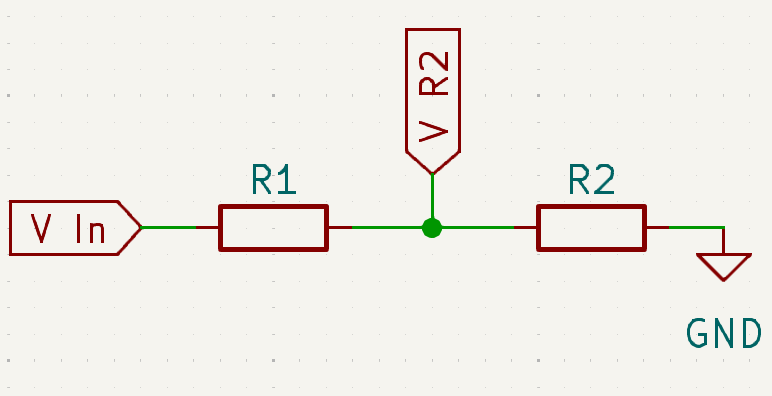
\includegraphics[width=0.6\textwidth]{figures/fig_voltage_divider.png}
    \caption{Simple voltage divider circuit used for resistance measurement.}
\end{figure}

Equations~\ref{eqn:voltage_divider} and~\ref{eqn:resistance_divider} are used to calculate the resistance from the voltage divider equation.
\begin{equation}\label{eqn:voltage_divider}
    V_{R2} = V_{In} \times \frac{R_2}{R_1 + R_2}
\end{equation}
\begin{equation}\label{eqn:resistance_divider}
    R_2 = \frac{R_1 \times V_{R2}}{V_{In}-V_{R2}}
\end{equation}


\section{Circuit Design}
The probe circuit is the circuit which contains the resistor divider, was designed to be printed onto a \gls{pcb}.
This design was influenced by Reference~\cite{cam_clark}, where a similar device was designed for salinity measurements in ice columns.
A \gls{pcb} was chosen for this circuit as the researcher had significant experience with \gls{pcb} design, and the manufacturing process offered higher precision than hand soldering, and is relatively cost-effective.
Significant improvements and modifications were made to the resistor divider circuit, to allow for a wider range of testing.

For input power, a \gls{dac} was used to drive the circuit. This allowed to the input voltage to be varied between $0 V$ and the referencevoltage, which was chosen to be $5V$.
This allowed for a range of voltages to be applied, which allowed for the measurement of the water's voltage-resistance relationship, and the creation of \gls{ac} signals.
A function generator was considered for generating the \gls{ac} signal, as it would allow for signals of a wider frequency and and high precision, however the price could not be accomodated by the budget.
The choice of \gls{dac}, and all following components, was first influenced by availability on JLCPCB, the \gls{pcb} manufacturing house.
The MCP4725 was chosen for its high resolution of 12-bits, offering a digital range of 0-4095, fast update time of $6{\mu}s$, and interface speed of 3.4MHz.
These features allow for both \gls{dc} and \gls{ac} signal analysis.

An op-amp with unity gain was the connected to the output of the \gls{dac}.
This is because \gls{dac}s have limited output drive capabilities, and the op-amp would allow for heavier loads to be driven.
Additionally the op-amp offers improved output stability, introduces impedance isolation, which protects the \gls{dac} from load variations and feedback effects, and allows for better sine wave quality.

As mentioned in Section~\ref{sec:res_mes}, for the resistor divider circuit, the electrodes would serve as $R_2$ and a known resistor as $R_1$.
Three alernative values of $R_1$ were chosen, to accomodate for any circuit errors.
These could be switched between using the TS3A4751 multiplexer \gls{ic}.
This switching multiplexer was chosen, for its low on-state resistance of $0.9\Omega$, and fast switching speed of $4-5ns$~\cite{cam_clark}.

The $R_1$ resistor values were chosen to be $100\Omega$, $1K\Omega$ and $10K\Omega$.
These values would be used when the resistance between the probes was $1-10\Omega$, $10-100\Omega$, and $100-1K\Omega$ respectively.
Each \gls{ic} contained 4 switches.

For measuring the output resistor, the voltage over it was directed into a multiplying op-amp with a gain of 11.
This increases the resolution for the \gls{adc} readings, as low voltages may be hard to differentiate between when converted to digital data. 

This configuration would allow for a minumum resolution of $11\%$ of $V_{DAC}$ and maximum of $100\%$ of $V_{DAC}$, for the voltage measurement by the \gls{adc}, as shown in Equations~\ref{eqn:dac_11} and~\ref{eqn:dac_100}~\cite{cam_clark}.
Equations~\ref{eqn:dac_11} and~\ref{eqn:dac_100} show for the expected resistance of $7.55\Omega$ falling into the $1-10\Omega$ range.
However, if the resistance falls into the $10-100\Omega$, or $100-1K\Omega$, the respective $R_1$ resistors would be used and the maximum and minimum \gls{dac} resolutions would be the same.

\begin{equation}\label{eqn:dac_11}
    \frac{1\Omega}{1\Omega + 100\Omega}\times V_{DAC} \times 11 = 11\% V_{DAC}
\end{equation}

\begin{equation}\label{eqn:dac_100}
    \frac{10\Omega}{10\Omega + 100\Omega}\times V_{DAC} \times 11 = 100\% V_{DAC}
\end{equation}

The accuarcy of the $R_1$ resistor is integral to acheiving an accurate $R_2$ measurement.
The resistors available on JLCPCB had an acurracy of $\pm{1}\%$.
To increase the accuracy 3 equal resistors were put in parallel. This decreases the uncertainty of the total equivalent resistance~\cite{cam_clark}.
This is shown in Equations~\ref{eqn:parallel_r} to~\ref{eqn:resistance_uncertainty}.

\begin{equation}\label{eqn:parallel_r}
    R_{T} = {\left[{\sum_{i=1}^{n}{\frac{1}{R_n}}}\right]}^{-1}
\end{equation}

If all the Resistors are equal this simplifies to: 

\begin{equation}\label{eqn:parallel_r_equal}
    R_{T} = ({\frac{n}{R}})^{-1} = \frac{1}{n} \times R
\end{equation}

To propogate uncertainty the standard equation for combined uncertainty can be used: \\
\hspace*{2em}~If a quantity $y$ depends on several independent variables $x_1, x_2, \ldots, x_n$: \\
\hspace*{2em}~$y=f(x_1, x_2, ..., x_n)$ \\
\hspace*{2em}~and each $x_i$ has a standard uncertainty $u(x_i)$ then the combined standard uncertainty \\
\hspace*{2em}~of $y$, denoted $u_c(y)$, is:

\begin{equation}\label{eqn:standard_uncertainty}
    \delta_y=\sqrt{\sum_{i=1}^{n}{\left({{\frac{\partial{f}}{\partial{x_i}}}{\delta_{x_i}}}\right)}^2}
\end{equation}

For Resistance this can be shown as:

\begin{equation}\label{eqn:resistance_uncertainty}
    \delta_{R_T}=\sqrt{\sum_{i=1}^{n}{\left({{\frac{\partial{R_{T}}}{\partial{R}}}{\delta_{R}}}\right)}^2} = \sqrt{{\left({{\frac{1}{n}}\delta_R}\right)}^2} = \frac{1}{n}\delta_R
\end{equation}

Using the above equations, with resistors with an individual uncertainty of $\pm1\%$, three resistors in parallel have a combined uncertainty of $\pm0.33\%$
To created the intended $R_1$ resistances of $100\Omega$, $1K\Omega$ and $10K\Omega$, the three parallel resistors were chosen to use values of $300\Omega$, $3K\Omega$ and $30K\Omega$ respectively.

A second switch circuit was then used to configure the $R_2$ resistor.
With there being two electrodes, the switching circuit allowed for the user to choose which would be the anode and the cathode.
The switch also included a calibration resistor of $5\Omega$, which would allow for the calculation of the gain of the \gls{adc} when measuring.
This calibration resistor was also created using a parallel resistor configuration, where four $20\Omega$ resistors were connected in parallel to give the require resistance at an uncertainty of $\pm0.25\%$.

A simplified circuit diagram showing the resistance measuring circuit is shown in Figure~\ref{fig:resistance_circuit}.

\begin{figure}[H]\label{fig:resistance_circuit}
    \centering
    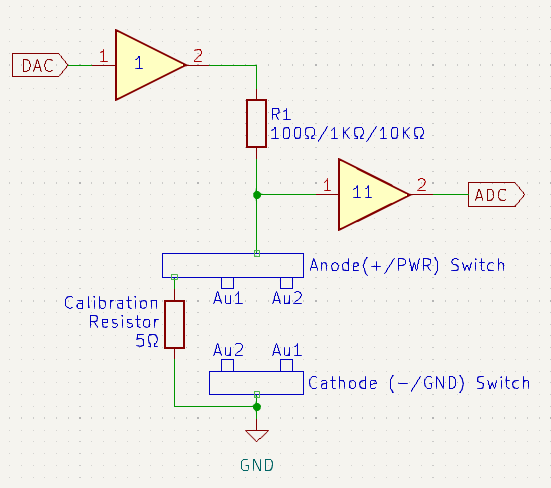
\includegraphics[width=0.75\textwidth]{figures/fig_resistance_circuit.png}
    \caption{Simple circuit diagram of the resistance measuring circuit.}
\end{figure}

A third switch was added to allow for the configuration of the fringe guard, allowing the fringe guard paired with an electrode to share the same voltage configuration, i.e.~when an electrode acted as the anode its fringe guard would also act as an anode, and vice versa.
The voltage of $R_1$ was directed through a unity gain buffer op-amp, and then connected on its output to the fringe guard, allowing for the same voltage over the electrodes to be over the fringe guards without affecting the measurement of the electrode voltage.

In addition to the resistance measuring circuitry, a waterproof pressure and temperature sensor was included, as these values are needed for calculating salinity.
The MS583702BA01-50 was chosen for its low price and availability on JLCPCB.
This sensor only allowed for up to 2 Bar pressure measurements, which was enough for this prototype, but would not satisfy the real-world requirements of the salinity probe.
Lastly, an RS-485 \gls(ic) was included for inter board communication.

A ESP-32 S2-Mini-2 was chosen for the microcontroller, as it was the most cost effective ESP32 based microcontroller.
It offered an FPU, allowing for the complex salinity calculations to be done, did not require a \gls{uart} bridge as it has built-in USB OTG support, allowing it to connect directly to a computer for easy programming, and offered 13-bit \gls{adc}s, allowing for a good voltage measurement resolution.
The researcher also had significant experience with this microcontroller.

A Controller \gls{pcb} was designed alongside the probe \gls{pcb}.
This controller was designed to communicate with the probe while it was submerged, sending it instructions and receiving results.
It allowed for the measurements to be recorded in a $.txt$ file on a micro-SD card, and displayed on a $16\times2$ LCD screen.
The \gls{pcb} for this controller was minimal, and relied on external breakout circuit boards.
This was due to budget constraints, and did not affect the effectiveness of the controller.
Only the voltage regualtion circuitry, and inter-board communication (RS-485) \gls{ic} were included in the production.
Headers were included on the controller \gls{pcb} to allow an ESP-Wroom-32 to be mounted to it.
Additional headers were included to allow the breakout boards for the LCD display and SD card reader to connect to the ESP32. 

For the inter-board connection the RS-485 communication protocol was chosen.
The ESP32 microcontrollers do support wireless communication through bluetooth and Wi-Fi.
However, 
